\appendix

\section{Tagging procedure}
\label{Taggingprocedure}

The following description is adopted from \citet{Verhelst2018}. 100 Eels were caught and tagged at the tidal weir in Merelbeke in the Zeeschelde during late summer and autumn (September–November) of three consecutive years (2015 till 2017) using double fyke nets. After periods of heavy rain, water flows over the sluices allowing eels to swim over the sluices. Placing the fyke nets behind the sluices and during periods of heavy rain, allowed to coordinate capture events and improve the chance of capturing eel. Several morphometric features were measured in order to determine the eel maturation stage \citep{Durif2005}: Total length (TL, to the nearest mm), body weight (W, to the nearest g), the vertical and horizontal eye diameter (EDv and EDh respectively, to the nearest 0.01 mm) and the length of the pectoral fin (FL, to the nearest 0.01 mm) (Table \ref{eel_morph}). Only females were tagged, since males are smaller than the minimum size handled in this study (< 450 mm \citep{Durif2005}). Eels of three different maturation stages were tagged: premigrant (F3, n = 51) and the two migrant stages F4 and F5 (n = 21 and n = 28, respectively). The eels were tagged with V13 coded acoustic transmitters (13 x 36 mm, weight in air 11 g, frequency 69 kHz, ping frequency: 60–100 s; estimated battery life: 1021-1219 days (battery life time depended on specific transmitter settings), (Table \ref{settingsTaggedEels})) from VEMCO Ltd (Canada). After anaesthetizing them with 0.3 ml/L clove oil, tags were implanted with permanent monofilament \citep{Thorstad2013b}. Eels recovered in a quarantine reservoir for approximately one hour and were subsequently released at the nearest receiver. 

\setcounter{table}{0} \renewcommand{\thetable}{A.\arabic{table}}

\renewcommand{\arraystretch}{1.5}
\begin{table}[]
\centering
\scriptsize
\caption{Number of all tagged female eels per stage with the different morphometrics: total length (TL), body weight (BW), horizontal and vertical eye diameters (EDh and EDv, respectively) and pectoral fin length (FL). Mean, standard deviation and range (between brackets) are indicated (Adopted from \citet{Verhelst2018}).}
\label{eel_morph}
\begin{tabular}{lllllll}
\toprule
Stage & Number & TL (mm)                                                         & BW (g)                                                             & EDh (mm)                                                               & EDv (mm)                                                              & FL (mm)                                                                 \\ \midrule
F3  & 51     & \begin{tabular}[c]{@{}l@{}}$702 \pm $57 \\ (568 - 835)\end{tabular} & \begin{tabular}[c]{@{}l@{}}$674 \pm $165 \\ (324 - 1106)\end{tabular}  & \begin{tabular}[c]{@{}l@{}}$8.08 \pm $0.57 \\ (6.77 - 9.08)\end{tabular}   & \begin{tabular}[c]{@{}l@{}}$7.55 \pm $0.60 \\ (6.20 - 9.70)\end{tabular}  & \begin{tabular}[c]{@{}l@{}}$32.92 \pm $3.29 \\ (26.76 - 40.32)\end{tabular} \\ 
F4   & 21     & \begin{tabular}[c]{@{}l@{}}$810 \pm $57 \\ (707 - 932)\end{tabular} & \begin{tabular}[c]{@{}l@{}}$1162 \pm $217 \\ (771 - 1830)\end{tabular} & \begin{tabular}[c]{@{}l@{}}$10.41 \pm $0.92 \\ (9.13 - 12.49)\end{tabular} & \begin{tabular}[c]{@{}l@{}}$9.66 \pm $0.78 \\ (8.60 - 11.86)\end{tabular} & \begin{tabular}[c]{@{}l@{}}$40.86 \pm $4.32 \\ (30.84 - 48.18)\end{tabular} \\ 
F5    & 28     & \begin{tabular}[c]{@{}l@{}}$662 \pm $56 \\ (575 - 775)\end{tabular} & \begin{tabular}[c]{@{}l@{}}$585 \pm $144 \\ (417 - 912)\end{tabular}   & \begin{tabular}[c]{@{}l@{}}$9.33 \pm $0.80 \\ (8.14 - 11.18)\end{tabular}  & \begin{tabular}[c]{@{}l@{}}$8.80 \pm $0.79 \\ (7.62 - 10.39)\end{tabular} & \begin{tabular}[c]{@{}l@{}}$34.41 \pm $3.68 \\ (28.97 - 45.37)\end{tabular} \\ \bottomrule
\end{tabular}
\end{table}
\renewcommand{\arraystretch}{1}

\renewcommand{\arraystretch}{1.25}
\begin{table}[]
\centering
\scriptsize
\caption{The number and settings of the transmitters of all tagged eels per step: power output (PO; L = low power output, H = high power output), ping frequency (s) and the time duration (days) per step as well as the total battery life time (days). (Adopted from \citet{Verhelst2018})}
\label{settingsTaggedEels}
\begin{tabular}{l|lll|lll|l} 
\toprule
\multirow{2}{*}{\begin{tabular}[l]{@{}l@{}}Number \\ of \\ transmitters \end{tabular}} & \multicolumn{3}{c|}{Step 1}                                                                                                          & \multicolumn{3}{c|}{Step 2}                                                                                                          & \multirow{2}{*}{\begin{tabular}[l]{@{}l@{}}Battery \\ life \\ (days) \end{tabular}}  \\
                                                                                       & PO & \begin{tabular}[l]{@{}l@{}}Ping \\ frequency  (s) \end{tabular} & \begin{tabular}[l]{@{}l@{}}Duration \\ (days) \end{tabular} & PO & \begin{tabular}[l]{@{}l@{}}Ping \\ frequency (s) \end{tabular} & \begin{tabular}[l]{@{}l@{}}Duration \\ (days) \end{tabular} &                                                                                      \\ 
\midrule
20                                                                                     & L  & 60 - 100                                                          & 1216                                                        & NA & NA                                                                & NA                                                          & 1216                                                                                 \\
40                                                                                     & H  & 60 - 100                                                          & 120                                                         & L  & 60 - 100                                                          & 901                                                         & 1021                                                                                 \\
40                                                                                     & H  & 60 - 100                                                          & 120                                                         & L  & 60 - 100                                                          & 902                                                         & 1022                                                                                 \\
\bottomrule
\end{tabular}
\end{table}
\renewcommand{\arraystretch}{1}

\section{Telemetry network}
\label{Telemetry_network}
\setcounter{table}{0} \renewcommand{\thetable}{B.\arabic{table}}

\renewcommand{\arraystretch}{1.25}
\begin{table}
\centering
\scriptsize
\caption{List of gates, with distance from Ghent (km), deployment date, number of included receivers, period of receiver inactivity and detection probability. Receiver inactivity represents the period during which one receiver of the gate was inactive. Adapted from \cite{Bruneel2020QuantifyingSystems}.}
\label{gate_list}
\begin{tabular}{c|ccccc} 
\toprule
\begin{tabular}[c]{@{}c@{}}gate\\name \end{tabular} & \begin{tabular}[c]{@{}c@{}}Distance\\(km) \end{tabular} & \begin{tabular}[c]{@{}c@{}}Deployment\\date \end{tabular} & \begin{tabular}[c]{@{}c@{}}Number\\of receivers \end{tabular} & Receiver inactivity          & \begin{tabular}[c]{@{}c@{}}Det. prob. \\(\%)\end{tabular}  \\ 
\midrule
s1                                                  & 0.0                                                     & 31/03/2015                                                & 1                                                       &                         & 100.0                                                                   \\ 
s2                                                  & 6.6                                                     & 20/03/2016                                                & 1                                                       &                         & 100.0                                                                   \\ 
s3                                                  & 12.1                                                    & 20/03/2016                                                & 1                                                       &                         & 97.1                                                                    \\ 
s4                                                  & 16.8                                                    & 20/04/2015                                                & 1                                                       &                         & 97.4                                                                    \\ 
s5                                                  & 26.7                                                    & 31/03/2015                                                & 1                                                       &                         & 99.1                                                                    \\ 
s6                                                  & 30.6                                                    & 2/04/2015                                                 & 1                                                       &                         & 98.7                                                                    \\ 
s7                                                  & 33.0                                                    & 24/03/2016                                                & 1                                                       & 17/10/2017 - 24/11/2017 & 96.7                                                                    \\ 
s8                                                  & 39.3                                                    & 24/03/2016                                                & 1                                                       &                         & 81.6                                                                    \\ 
s9                                                  & 40.8                                                    & 20/04/2015                                                & 1                                                       &                         & 99.9                                                                    \\ 
s10                                                 & 44.1                                                    & 20/04/2015                                                & 1                                                       &                         & 99.3                                                                    \\ 
s11                                                 & 46.5                                                    & 27/04/2015                                                & 1                                                       &                         & 100.0                                                                   \\ 
s12                                                 & 49.0                                                    & 2/04/2015                                                 & 1                                                       &                         & 98.4                                                                    \\ 
s13                                                 & 53.8                                                    & 2/04/2015                                                 & 1                                                       &                         & 93.2                                                                    \\ 
s14                                                 & 55.6                                                    & 2/04/2015                                                 & 1                                                       &                         & 100.0                                                                   \\ 
s15                                                 & 63.3                                                    & 2/04/2015                                                 & 2                                                       &                         & 100.0                                                            \\ 
s16                                                 & 68.6                                                    & 2/04/2015                                                 & 2                                                       &                         & 100.0                                                            \\ 
s17                                                 & 75.8                                                    & 30/09/2015                                                & 3                                                       &                         & 100.0                                                               \\ 
s18                                                 & 88.2                                                    & 3/09/2015                                                 & 2                                                       &                         & 77.8                                                             \\ 
ws1                                                 & 112.8                                                   & 22/09/2015                                                & 6                                                       &                         & 91.3                                                             \\ 
                                         
\bottomrule
\end{tabular}
\end{table}
\renewcommand{\arraystretch}{1}

\section{Figures}
\setcounter{figure}{0} \renewcommand{\thetable}{C.\arabic{table}}
\begin{figure}[h!]
  \centering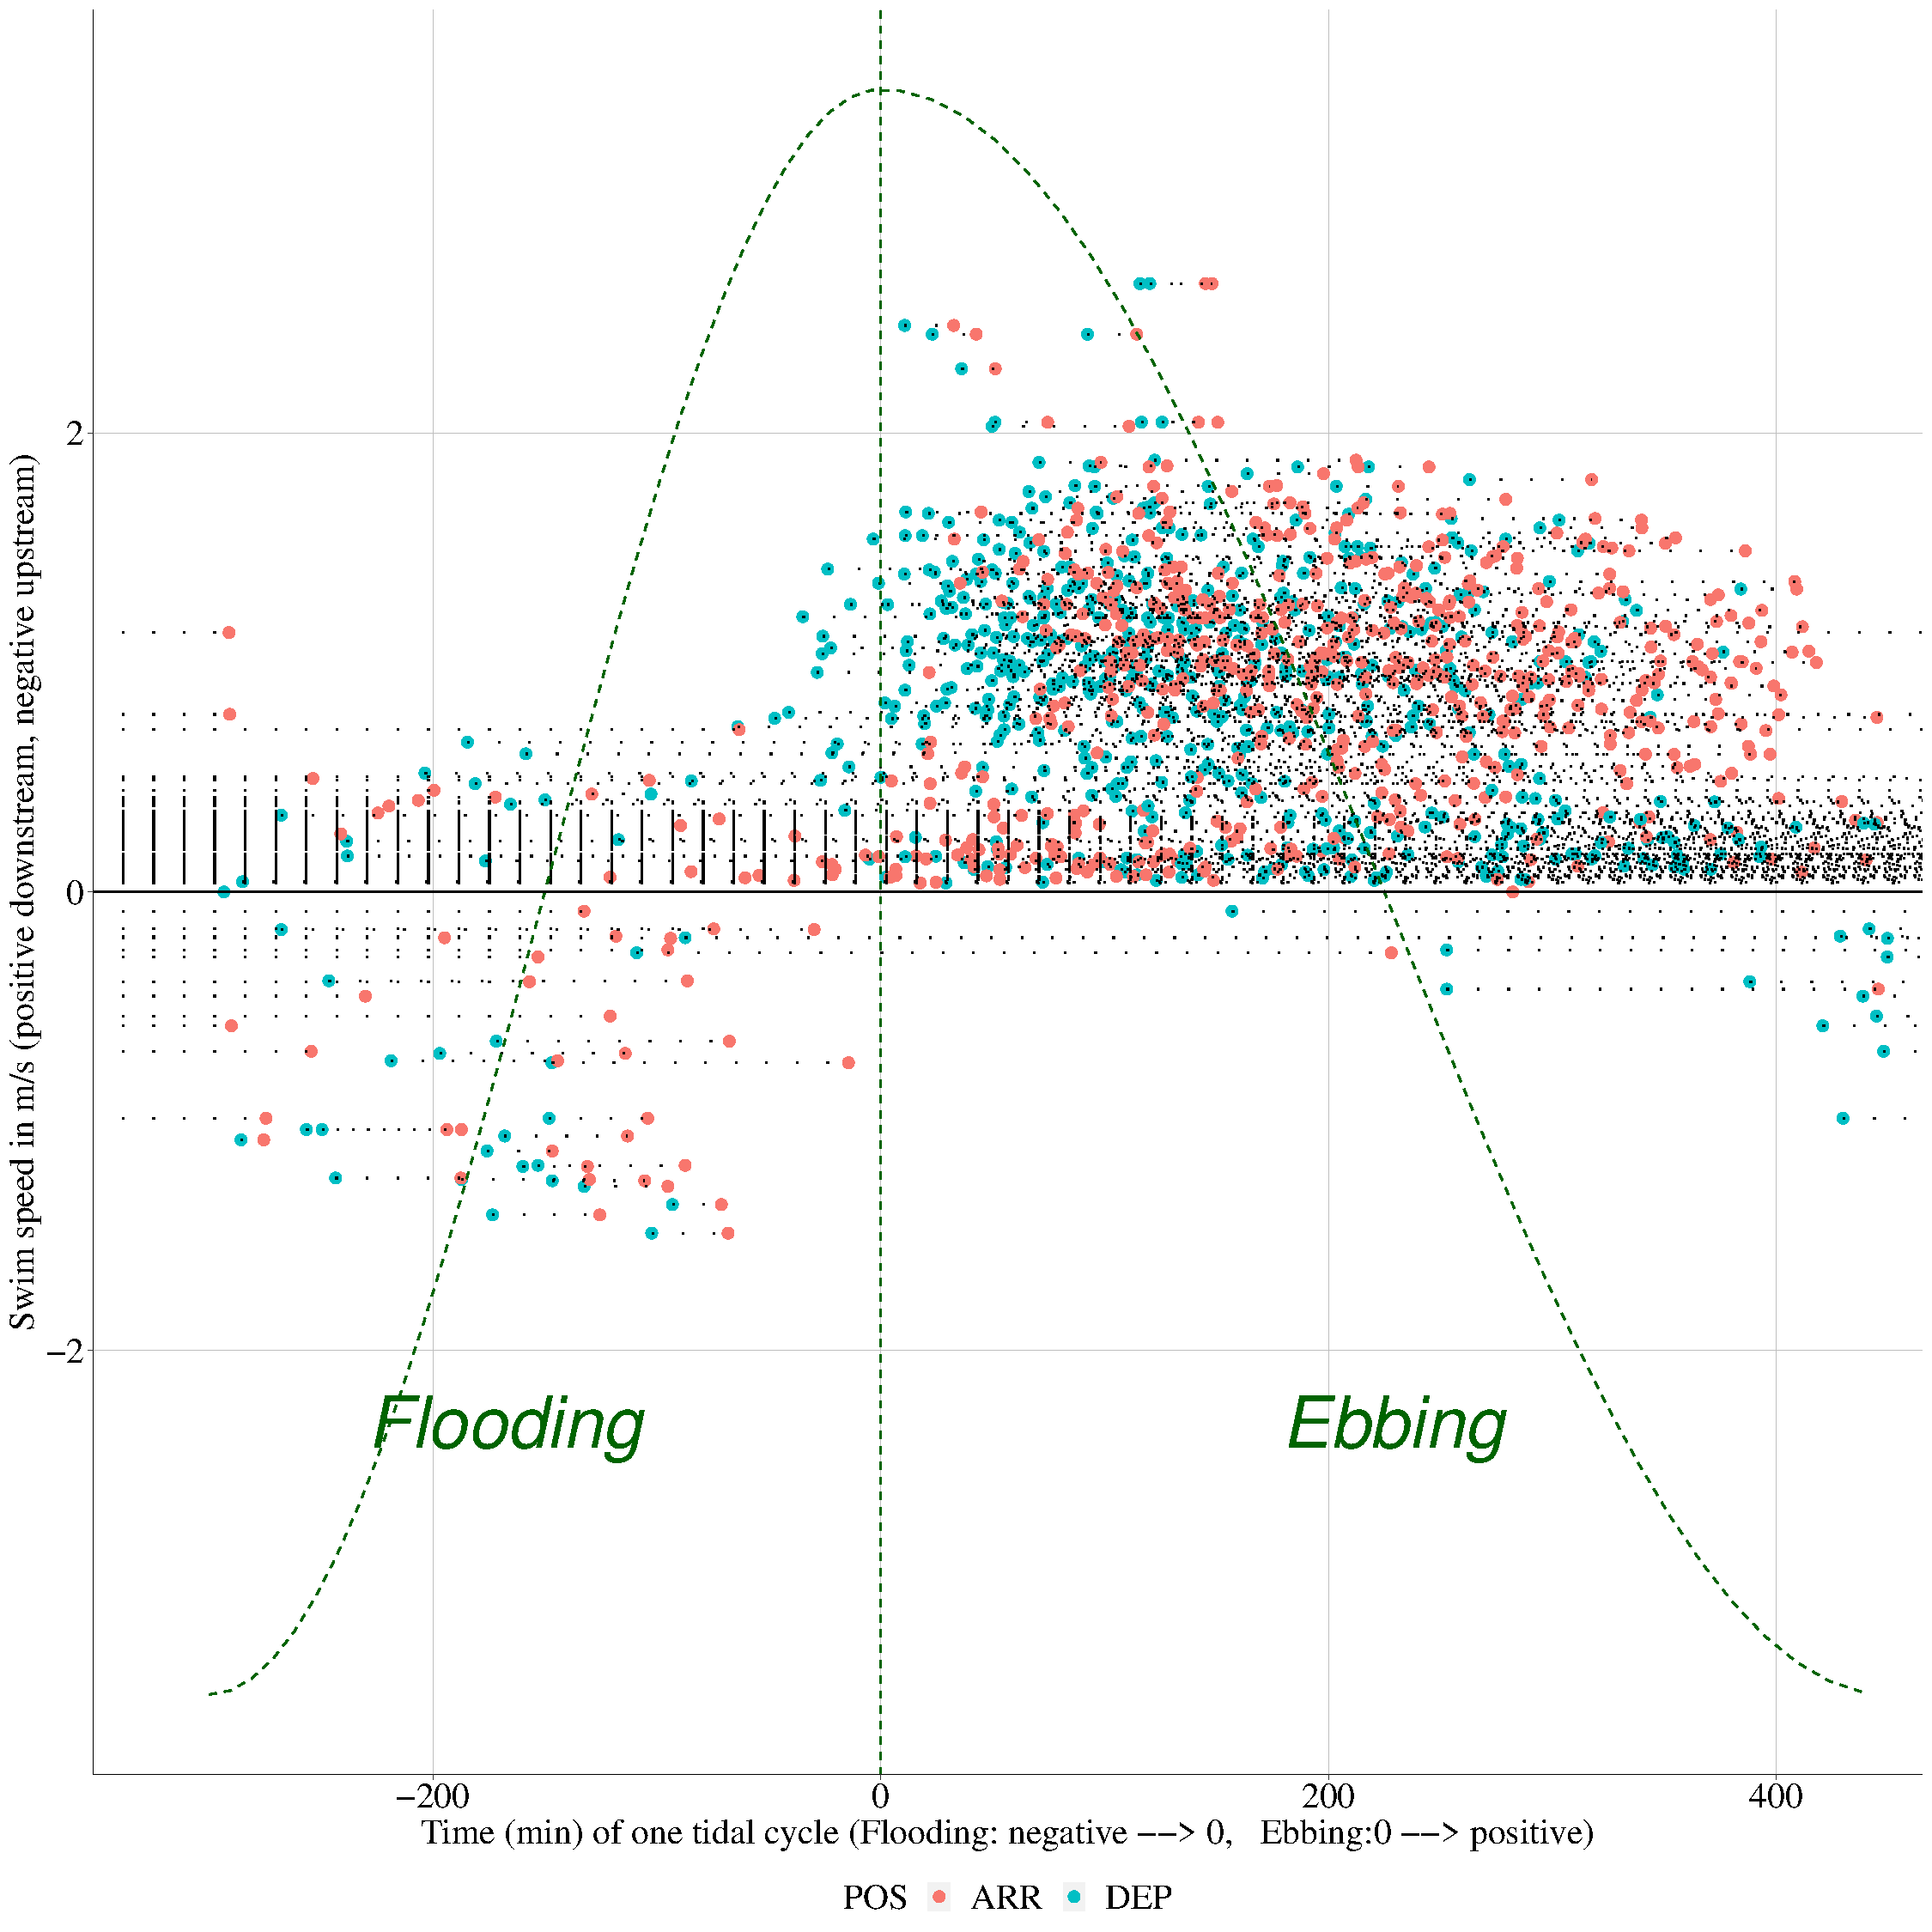
\includegraphics[scale=0.35]{Departure_and_arrival.pdf}
  \caption{Movement intervals of all tagged eels depicted by the departure (DEP) from a receiver and arrival (ARR) at another receiver. The swimming speed (m s$^{-1}$) during a movement interval is given in function of the moment within the tidal cycle. In the ZS, the period of ebbing is larger than the period of flooding, with differences being most pronounced upstream. However, for visualization purposes the average period of flooding (300 minutes) and period of ebbing (450 minutes) of the city of Dendermonde (in the center of the ZS) were used to rescale the TMIs \citep{Levy2014HetGetijkarakteristieken}
  }
  \label{Departure_and_arrival}
\end{figure}
